\documentclass[12pt,a4paper]{article}
\usepackage[utf8]{inputenc}
\usepackage[T1]{fontenc}
\usepackage{graphicx}
\usepackage{hyperref}
\usepackage{listings}
\usepackage{xcolor}
\usepackage{tikz}
\usepackage{float}
\usepackage[margin=2.5cm]{geometry}

% Define colors for code and architecture diagram
\definecolor{codegreen}{rgb}{0,0.6,0}
\definecolor{codegray}{rgb}{0.5,0.5,0.5}
\definecolor{codepurple}{rgb}{0.58,0,0.82}
\definecolor{backcolour}{rgb}{0.95,0.95,0.92}

% Code listing style
\lstdefinestyle{mystyle}{
    backgroundcolor=\color{backcolour},   
    commentstyle=\color{codegreen},
    keywordstyle=\color{magenta},
    numberstyle=\tiny\color{codegray},
    stringstyle=\color{codepurple},
    basicstyle=\ttfamily\footnotesize,
    breakatwhitespace=false,         
    breaklines=true,                 
    captionpos=b,                    
    keepspaces=true,                 
    numbers=left,                    
    numbersep=5pt,                  
    showspaces=false,                
    showstringspaces=false,
    showtabs=false,                  
    tabsize=2
}
\lstset{style=mystyle}

\title{Container Monitoring System with Message Queue\\Technical Report}
\author{
    Group Members:\\
    Yassin ES SAIM\\
    Malik MOUSSA\\
    Laurine Collin DUFRENSE\\
    Nikita SIDARENKA
    \\
    \href{https://github.com/laurinecd/SoftwareArchiPRoject.git}{GitHub Repository}
}
\date{\today}

\begin{document}

\maketitle

\section{Introduction and Context}

In modern distributed systems, effective monitoring is crucial for maintaining system reliability and performance. Our project implements a message queue-based system with two essential monitoring features that address common challenges in containerized environments.

\section{Feature 1: Container Health Monitoring with Discord Alerts}

\subsection{Problem Statement and Motivation}
In containerized environments, system failures can occur silently, leading to service disruptions that may go unnoticed. Traditional monitoring solutions often lack immediate notification capabilities or require constant dashboard observation. We identified the need for:
\begin{itemize}
    \item Instant awareness of container failures
    \item Automated recovery procedures
    \item Historical tracking of system stability
\end{itemize}

\subsection{Implementation Approach}
Our solution leverages Discord's widespread adoption in development teams to create an effective alert system. The implementation consists of several interconnected components:

\subsubsection{Alert Configuration}
We implemented a Prometheus-based alert configuration that monitors container status:
\begin{lstlisting}[language=yaml]
apiVersion: 1
groups:
  - name: ContainerAlerts
    rules:
      - uid: container_down
        title: Container Down
        condition: B
        data:
          - refId: A
            datasourceUid: prometheus
            model:
              expr: up{job=~"app1|app2"} < 1
\end{lstlisting}

This configuration enables:
\begin{itemize}
    \item Real-time status monitoring of critical containers
    \item Customizable alert conditions based on container metrics
    \item Integration with Grafana's alerting system
\end{itemize}

\subsubsection{Discord Integration Architecture}
The Discord notification system was designed with reliability in mind:
\begin{itemize}
    \item \textbf{Webhook System}: Secure, token-based authentication
    \item \textbf{Message Format}: Structured alerts with severity levels and timestamps
    \item \textbf{Retry Logic}: Exponential backoff for failed notifications
    \item \textbf{Error Handling}: Comprehensive logging of notification failures
\end{itemize}

\newpage

\section{Feature 2: Message Queue Monitoring with Grafana and Prometheus}

\subsection{Problem Statement and Motivation}
Message queues in distributed systems can become bottlenecks, with issues often discovered too late. Our Grafana dashboard addresses:
\begin{itemize}
    \item Lack of visibility into message processing
    \item Difficulty in identifying performance bottlenecks
    \item Complex correlation between system metrics
    \item Need for historical performance analysis
\end{itemize}

\subsection{Technical Implementation}

\subsubsection{Grafana and Prometheus Integration}
We implemented a comprehensive monitoring stack that includes:
\begin{itemize}
    \item \textbf{Prometheus}: For metrics collection, storage, and querying
    \item \textbf{Grafana}: For visualization and alerting capabilities
\end{itemize}

Our architecture allows real-time monitoring of all message queue components while maintaining historical data for trend analysis.

\subsubsection{Dashboard Architecture}
The Grafana dashboard provides comprehensive visualization of our message queue metrics:

\begin{figure}[H]
\centering
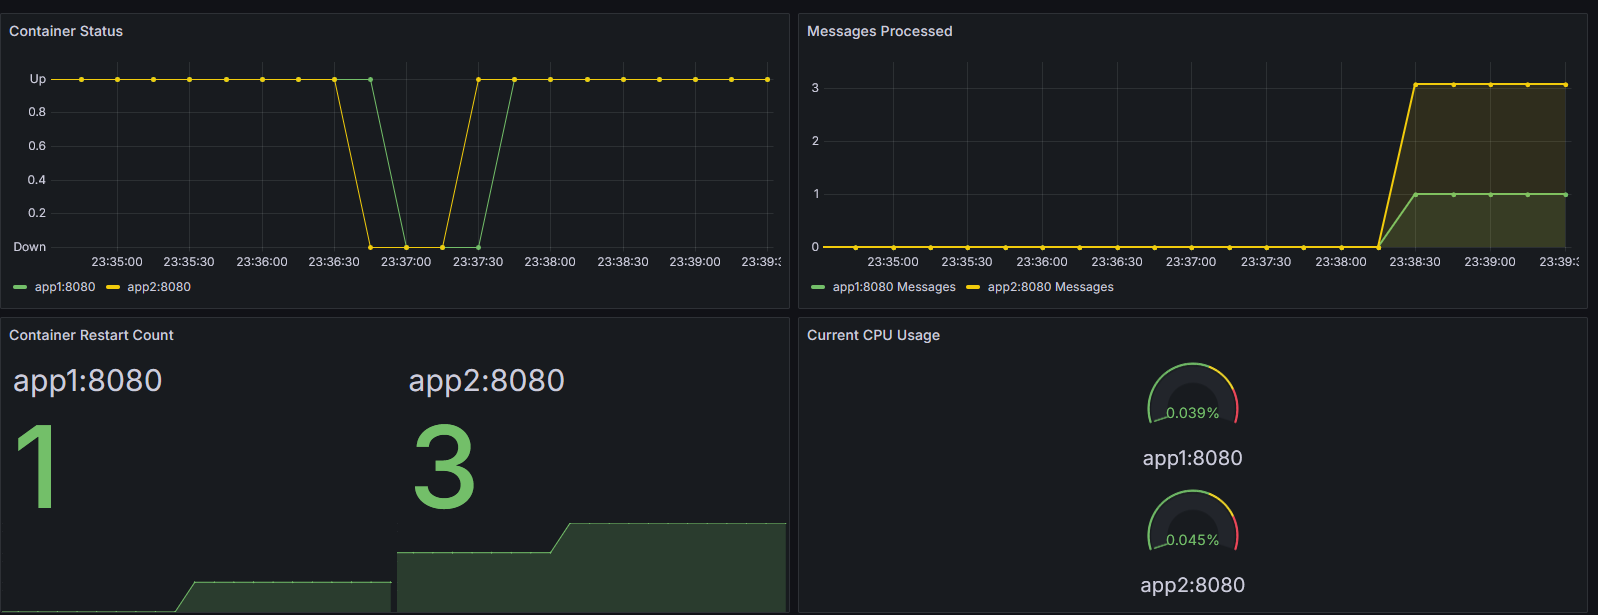
\includegraphics[width=0.9\textwidth]{image.png}
\caption{Grafana Dashboard for Message Queue Monitoring}
\end{figure}

\subsubsection{Prometheus Metrics Implementation}
Our metrics collection system uses Spring's scheduling capabilities with Prometheus integration:
\begin{lstlisting}[language=java]
@Scheduled(fixedRate = 5000)
public void collectMetrics() {
    // Message processing metrics with Prometheus collectors
    messageCounter.increment();
    processingTime.record(duration);
    queueDepth.set(currentDepth);
    
    // Prometheus-based error tracking
    if (hasError) {
        errorCounter.increment();
        failureGauge.set(errorCount);
        logErrorDetails(error);  // Enhanced error logging
    }
}
\end{lstlisting}

The integration with Prometheus allows us to:
\begin{itemize}
    \item Create custom alerts based on complex conditions
    \item Track message processing rates and error percentages
    \item Monitor queue depths to prevent overflow conditions
    \item Correlate service performance with message processing metrics
\end{itemize}


\section{Conclusion}

The combination of container health monitoring and Grafana/Prometheus-based message queue visualization has created a robust monitoring solution. Key achievements include:
\begin{itemize}
    \item Seamless integration of monitoring and alerting
    \item Real-time visibility into system performance
    \item Proactive issue detection and resolution
    \item Comprehensive system health management
\end{itemize}

\end{document}